% Copright (C) 2014 Daniil Baturin <daniil at baturin dot org>
%
% This work is licensed under the Creative Commons Attribution-ShareAlike 4.0 International License.
% To view a copy of this license, visit http://creativecommons.org/licenses/by-sa/4.0/.

\chapter{Routing overview}

Network routing is the process of determining packet path.

\section{Network addressing}

Internets consist of hosts and every host is identified by a unique address. A network address is an unsigned integer number.
Different versions of the IP protocol use different address size, IPv4 addresses are 32 bit, and IPv6 addresses are 128 bit long.

Hosts are organized into networks, for that purpose hosts from the same group are assigned with an addresses from a contiguous block
of addresses starting with the same bit sequence. The common part of those addresses is known as a \emph{network address}.

It would be extremely inefficient to store information about every single host, so all routing decisions
are taken in terms of networks. When a router receives a packet, it takes its destination address and
checks if it belongs to any of the networks the router knows about.

The network and host parts of an address are extracted by applying a \emph{bit mask} which is commonly referred to as 
a \emph{subnet mask} in network addressing context.

Suppose we are using $11111111111111111111111100000000_2$ as a mask (255.255.255.0 in dotted decimal format).
This allows for 256 hosts in a network by extracting network and host parts from a 192.0.2.44 address ($1100000000000  0000000001000101100_2$ in binary).

We can use bitwise logical AND operations that keep bits at positions where the mask bits are set to 1 intact and zeroes the rest.

\begin{tabular}{|l|l|l|}
\hline
AND & 0 & 1 \\
\hline
0 & 0 & 0 \\
\hline
1 & 0 & 1 \\
\hline
\end{tabular}

So we can state that 
\begin{equation}
  network\ address = address\ \mathrm{AND}\ mask
\end{equation}

Different networks have a different number of hosts, which requires a way to split the address space into chunks of
different sizes, and a way to determine how many bits of an address identify the network, and how many bits
identify the host within that network.

In the early Internet this problem was solved by the introduction of \emph{address classes}. The value of the first
bits of the addresses used to define its class, and the class used to define network size.

\begin{tabular}{|l|l|l|l|l|}
\hline
Class & First bits & Size & First network & Last network \\
\hline
A & 0000 & 16,777,216 ($2^{24}$) & 0.0.0.0 & 127.0.0.0 \\
\hline
B & 1000 & 65 536 ($2^{16}$) & 128.0.0.0 & 191.255.0.0 \\
\hline
C & 1100 & 256 ($2^{8}$) & 192.0.0.0 & 223.255.255.0 \\
\hline
D & 1110 & Not defined & Not defined & Not defined \\
\hline
E & 1111 & Not defined & Not defined & Not defined \\
\hline
\end{tabular}

As the Internet grew in size, this approach was proven inefficient. Networks with more than 256 hosts had to
request class B networks that were often too large for them and most of addresses were unused. Every single
network had to be present in the global routing table which inflated routing table size. There was no way
to split a network in parts to optimize internal routing.

\subsection{Classless addressing}

The current network addressing scheme is known as "classless addressing". The routing approach that is based on it
is called "classless interdomain routing" (CIDR). The addressing scheme is often referred to as CIDR as well.

A CIDR-formatted address consists of two parts: address and prefix length, separated by "/", such as
"2001:db8::1/64" or "192.0.2.10/24". Prefix length is a decimal number that defines how many bits are used
for the network part of the address.




\section{Routing tables}

Every system (either host or router) keeps a \emph{routing table} that contains \emph{routes} to known prefixes.

A route is a record that may include the following fields:
\begin{itemize}
  \item destination network address (prefix);
  \item next hop address;
  \item outbound interface;
  \item route metric;
  \item metainformation, such as protocol the route is learnt from.
\end{itemize}

An excerpt from a routing table may look like:
\begin{verbatim}
Codes: K - kernel route, C - connected, S - static, R - RIP, O - OSPF,
       I - ISIS, B - BGP, > - selected route, * - FIB route

S>* 0.0.0.0/0 [210/0] via 192.0.2.1, eth0
C>* 192.0.2.0/24 is directly connected, eth0
S>* 203.0.113.0/24 [1/0] via 192.0.2.10, eth0
S>* 203.0.113.128/25 [1/0] via 192.0.2.11, eth0
\end{verbatim}

In the first entry, "S" means the route is statically configured, which is metainformation;
0.0.0.0/0 is the destination prefix; 192.0.2.1 is the next hop address; and eth0 is the
outbound interface.

The routing table is traversed from less specific to more specific routes. The route selection algorithm follows the "longest match" rule: if more than one route matches the destination,
the most specific one is used.

Suppose the above system receives a packet destined to 203.0.113.250. It matches the 0.0.0.0/0
destination (as any other possible address), but there is a route to 203.0.113.0/24, which is
more specific. Furthermore, there is a route to 203.0.113.128.0/25, which is even more specific.
The table does not have any more specific routes, so the route with the 203.0.113.128/25 prefix 
will be used.

If the system had a route with e.g. 201.0.113.250/32 prefix in addition to those ones, it would
be used for the routing decision for that packet.



\section{Connected routes}


\section{Dynamic routing and route lifecycle}

Configuring all routes statically quickly becomes unmanageable even in moderately large networks.
If you have several routers, in order to add, remove, or change a route you need to update the 
configuration on each router. This is tedious and error prone. For this reason dynamic routing
protocols were invented.

Routing protocols serve purposes: they exchange routing information between systems and
perform initial best path selection. When a new route appears in one system, it is advertised
to all others, and if a route becomes unavailable, it is automatically withdrawn from the routing tables.

Dynamic routing does not replace static routing, but complements it. A system may have both
statically configured and dynamically learned routes.

Typical architecture of a router includes the following components:

\begin{itemize}
\item Routing protocol processes
\item Routing Internet Base (RIB)
\item Forwarding Internet Base (FIB)
\end{itemize}

Together routing protocol processes and the RIB process form a \term{routing control plane}.
The FIB is used by a \term{forwarding plane}. A forwarding plane may be implemented in software
or hardware, while a control plane is always implemented in software.

\begin{figure}[h]
    \centering
    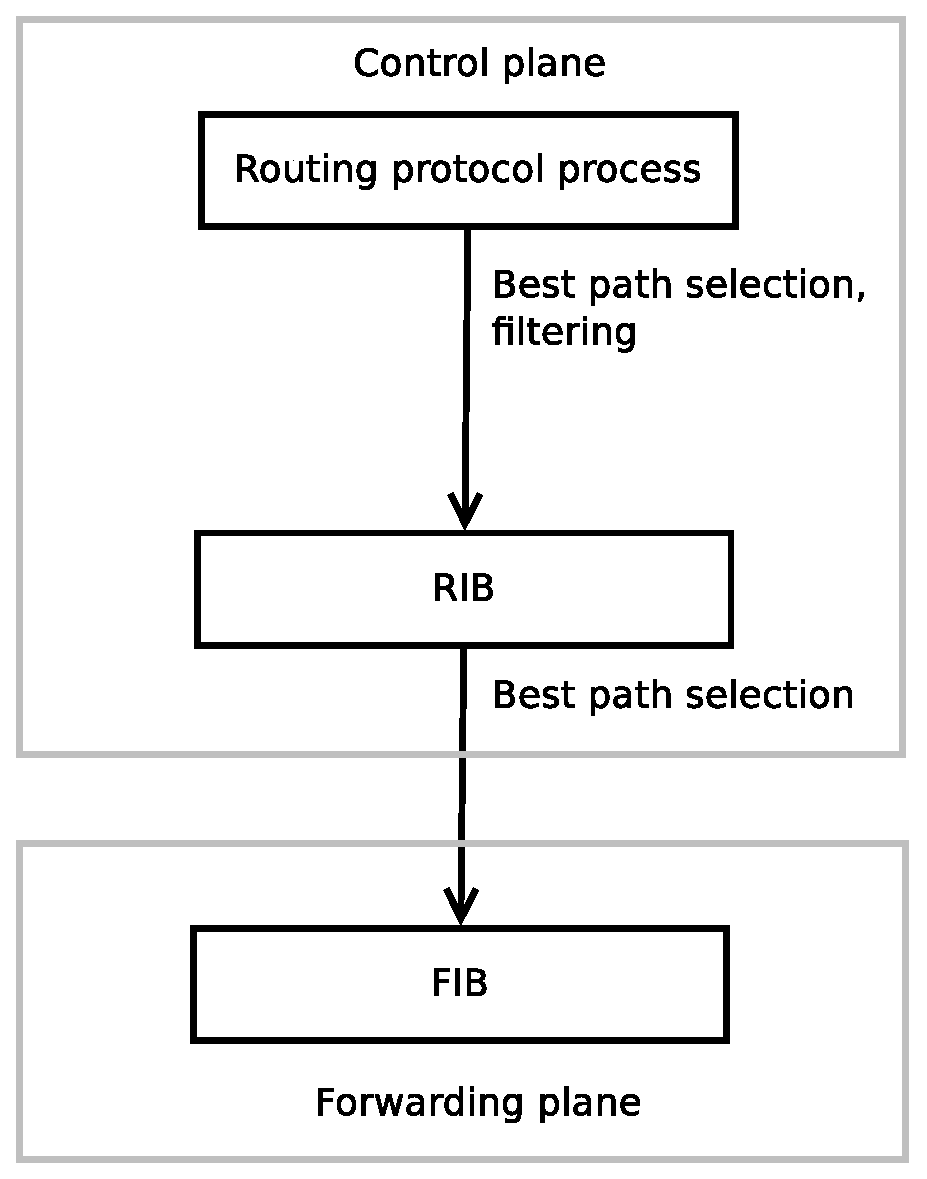
\includegraphics[width=0.5\textwidth]{graphics/router_architecture.eps}
    \caption{Router architecture}
    \label{fig:router_architecture}
\end{figure}

Every routing protocol process maintains its own route table that only contains routes learned
from the protocol it handles. If there is more than one route to the same destination, it
chooses the best of those routes and sends it to the RIB. It also receives routes that
are to be advertised to peers from the RIB.

The RIB collects all routes received from routing protocol processes. It then chooses the best
routes to every destination and sends the to the FIB. Thus if there are routes to the same
destination learned from different protocols, the best of those will be used. Static routes
are configured directly in the RIB and are also considered in the best path selection process,
as well as connected routes.

The forwarding plane performs actual packet forwarding according to the FIB routes.

In a Linux/Quagga stack, bgpd, ospfd etc. are routing protocol processes, zebra is the RIB,
and the Linux kernel is the forwarding plane.

\subsection{Administrative distance}

As mentioned above, the RIB chooses the best route from those supplied by the routing 
protocol processes, static routes, and connected routes. However, it needs some criteria
for choosing between those routes.

Routes are sorted by administrative distance. Administrative distance is a number that
defines how preferrable routes learned from some protocol are. Unless you have changed it
in the Quagga configuration, the defaults are:

\ \\

\noindent{}\begin{tabular}{ll}
\hline
Connected & 0 \\
Static & 1 \\
eBGP & 20 \\
OSPF & 110 \\
ISIS & 115 \\
RIP (and RIPng) 120 \\
iBGP & 200 \\
\hline
\end{tabular}

\ \\

Values for dynamic routing protocols can be arbitrary, but the order of connected
and static routes is important. Connected routes should always come first, since
they define gateway reachability. Static routes are often used to override dynamically
learned routes, so they should also come first.
